\documentclass{article}
\usepackage{ctex}
\usepackage{amsmath}
\usepackage{graphicx}
\usepackage{hyperref}
\usepackage{caption}
\usepackage{subcaption}
\usepackage{listings}
\usepackage{xcolor}
\usepackage{float} 


\lstset{
    basicstyle=\ttfamily,
    keywordstyle=\color{blue},
    commentstyle=\color{gray},
    stringstyle=\color{red},
    frame=single,
    breaklines=true
}

\title{Radon Transform and Image Reconstruction}
\author{王润泽}
\date{\today}

\begin{document}
\maketitle

\section{引言}
本实验的目的是实现 Radon 变换及其反变换,以重建图像。Radon 变换是一种数学技术,广泛应用于医学成像(如 CT 扫描)中,通过对图像进行投影来获取其内部结构的信息。

\section{实验目的}
本实验分为两部分:
\begin{enumerate}
    \item 实现没有滤波的 Radon 变换投影重建,重现课本图 5.39、图 5.40 的结果。
    \item 对比加汉明窗和不加汉明窗滤波器的效果,重现课本图 5.43 和图 5.44 的结果。
\end{enumerate}

\section{方法}
实验主要分为以下几个步骤:
\begin{enumerate}
    \item 使用 Radon 变换将输入图像转化为投影。
    \item 对投影进行傅里叶变换,并应用滤波器。
    \item 使用反投影方法重建图像。
\end{enumerate}

\subsection{Radon 变换}
Radon 变换的核心代码如下所示:

\begin{lstlisting}[language=Python]
import numpy as np
from scipy.fft import fft, ifft, fftfreq

def transform(image):
    size = image.shape
    round_size = int(np.sqrt(size[0]**2 + size[1]**2))
    result = np.zeros((180, round_size), dtype=int)

    for angle_ in range(180):
        for round in range(-round_size//2, round_size//2 + 1):
            if np.abs(angle_ - 90) > 45:
                angle = np.deg2rad(angle_)
                x = np.arange(size[0])
                y_ = -x + size[0] / 2

                x_ = round / np.cos(angle) - y_ * np.tan(angle)
                y = (x_ + size[1] / 2).astype(int)

                valid_mask = (y >= 0) & (y < size[1])
                result[angle_][round + (round_size // 2) - 1] += image[x[valid_mask], y[valid_mask]].sum()
            else:
                angle = np.deg2rad(angle_)
                y = np.arange(size[1])
                x_ = (y - size[1] / 2).astype(int)
                y_ = round / np.sin(angle) - x_ / np.tan(angle)
                x = (-y_ + size[0] / 2).astype(int)
                valid_mask = (x >= 0) & (x < size[0])
                    
                result[angle_][round + (round_size // 2) - 1] += image[x[valid_mask], y[valid_mask]].sum()

    # 结果缩放
    min_val = np.min(result)
    max_val = np.max(result)

    if max_val > min_val:
        result_scaled = (result - min_val) / (max_val - min_val) * 255
    else:
        result_scaled = np.zeros_like(result, dtype=np.float64)

    result_new = result_scaled.astype(np.uint8)
    return result_new
\end{lstlisting}

\subsection{滤波与反投影}
在投影中,我们使用汉明窗进行滤波,代码如下:

\begin{lstlisting}[language=Python]
def create_filter(size, use_hamming=True):
    filter_ = np.abs(fftfreq(size))
    if use_hamming:
        hamming = 0.54 - 0.46 * np.cos(2 * np.pi * np.arange(size) / size)
        hamming = np.roll(hamming, size // 2)
        filter_ = filter_ * hamming
    return filter_

def apply_filter(projections, use_hamming=True):
    filtered_projections = np.zeros_like(projections, dtype=np.float64)
    filter_ = create_filter(projections.shape[1], use_hamming)

    for i in range(projections.shape[0]):
        projection = projections[i]
        projection_fft = fft(projection)
        filtered_projection_fft = projection_fft * filter_
        filtered_projections[i] = np.real(ifft(filtered_projection_fft))
    
    return filtered_projections
\end{lstlisting}

反投影过程的代码如下:

\begin{lstlisting}[language=Python]
@njit(parallel=True)
def inverse_radon_transform(image, filtered_projections):
    size = image.shape
    result = np.zeros(size, dtype=np.float64)

    for x in range(size[0]):
        for y in range(size[1]):
            x_ = y - size[1] / 2
            y_ = -x + size[0] / 2
            for angle_ in range(180):
                angle = np.deg2rad(angle_)
                cos = np.cos(angle)
                sin = np.sin(angle)
                rou = x_ * cos + y_ * sin
                rou = int(round(rou))
                
                if np.abs(rou) > filtered_projections.shape[1] // 2:
                    continue
                result[x][y] += filtered_projections[angle_][rou + filtered_projections.shape[1] // 2 - 1]

    min_val = np.min(result)
    max_val = np.max(result)

    if max_val > min_val:
        result_scaled = (result - min_val) / (max_val - min_val) * 255
    else:
        result_scaled = np.zeros_like(result, dtype=np.float64)

    result = result_scaled.astype(np.uint8)
    return result
\end{lstlisting}

\section{实验结果}
通过上述步骤,我们对图像进行了 Radon 变换、滤波和反投影重建。以下是实验结果图像的示例(图 5.39、图 5.40、图 5.43 和图 5.44):

\begin{figure}[H]
    \centering
    \begin{subfigure}{0.45\textwidth}
        
\includegraphics[width=\textwidth]{../result_1_2/vertical_rectangle_1.png}
        \caption{Radon 变换结果 (vertical rectangle)}
    \end{subfigure}
    \hfill
    \begin{subfigure}{0.45\textwidth}
        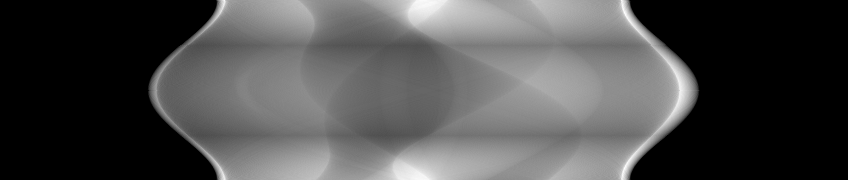
\includegraphics[width=\textwidth]{../result_1_2/shepp-logan_phantom_1.png}
        \caption{Radon 变换结果 (Shepp-Logan phantom)}
    \end{subfigure}
    
    \begin{subfigure}{0.45\textwidth}
        
\includegraphics[width=\textwidth]{../result_1_2/vertical_rectangle_2.png}
        \caption{反投影重建结果 (vertical rectangle)}
    \end{subfigure}
    \hfill
    \begin{subfigure}{0.45\textwidth}
        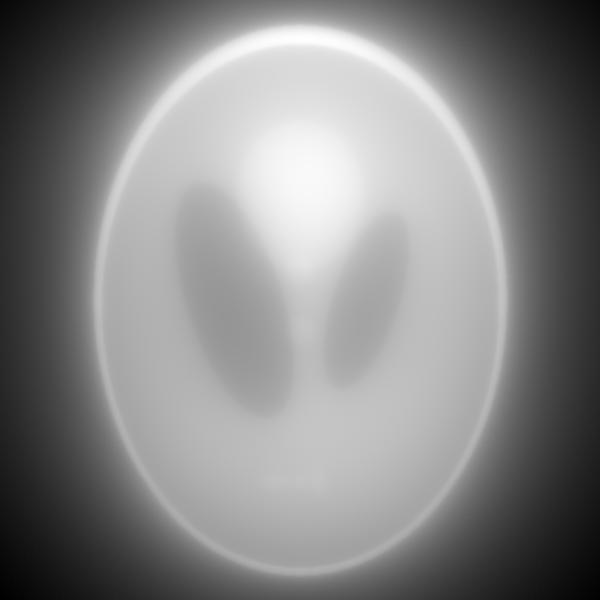
\includegraphics[width=\textwidth]{../result_1_2/shepp-logan_phantom_2.png}
        \caption{反投影重建结果 (Shepp-Logan phantom)}
    \end{subfigure}
    \caption{Radon 变换和反投影重建结果对比}
\end{figure}

\begin{figure}[H]
    \centering
    \begin{subfigure}{0.45\textwidth}
        
\includegraphics[width=\textwidth]{../result_3_4/vertical_rectangle_reconstructed_hamming.png}
        \caption{使用汉明窗重建的图像 (vertical rectangle)}
    \end{subfigure}
    \hfill
    \begin{subfigure}{0.45\textwidth}
        
\includegraphics[width=\textwidth]{../result_3_4/vertical_rectangle_reconstructed_no_hamming.png}
        \caption{不使用汉明窗重建的图像 (vertical rectangle)}
    \end{subfigure}
    
    \begin{subfigure}{0.45\textwidth}
        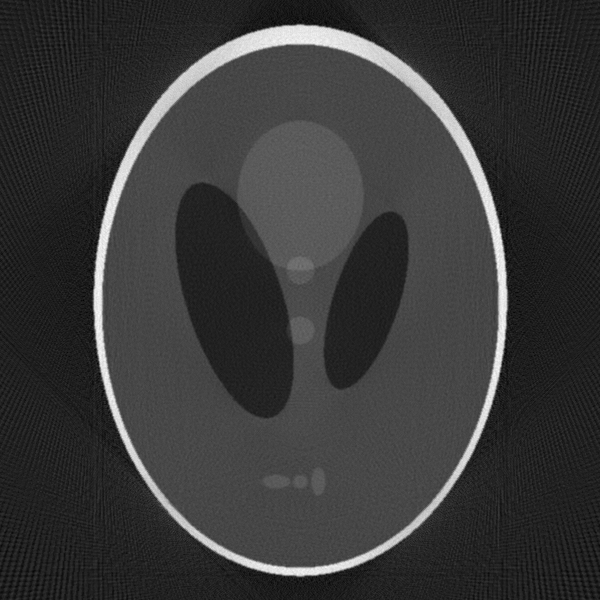
\includegraphics[width=\textwidth]{../result_3_4/shepp_logan_reconstructed_hamming.png}
        \caption{使用汉明窗重建的图像 (Shepp-Logan phantom)}
    \end{subfigure}
    \hfill
    \begin{subfigure}{0.45\textwidth}
        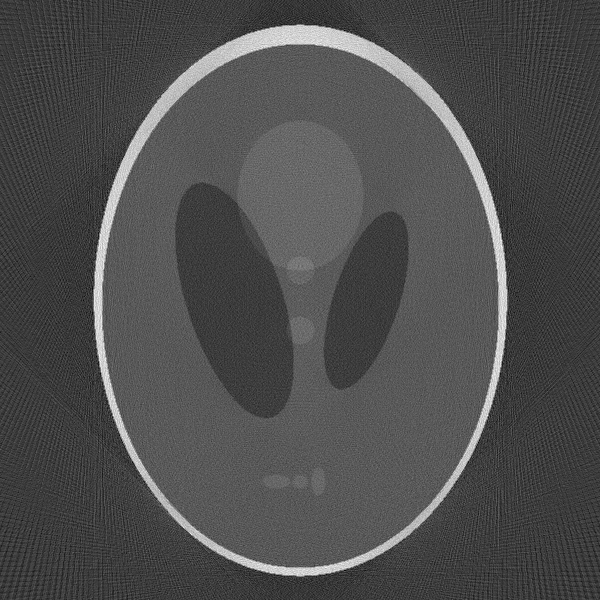
\includegraphics[width=\textwidth]{../result_3_4/shepp_logan_reconstructed_no_hamming.png}
        \caption{不使用汉明窗重建的图像 (Shepp-Logan phantom)}
    \end{subfigure}
    \caption{实验结果对比 (vertical rectangle 与 Shepp-Logan phantom)}
\end{figure}

\section{结论}
本实验成功实现了 Radon 变换及其反变换,验证了图像重建的有效性。使用汉明窗对投影进行滤波能够提高重建图像的质量,能有效缓解振铃效应,效果优于不使用窗函数的情况。

\end{document}
